% !TEX program = xelatex
\documentclass[12pt, a4paper]{article}
\usepackage[utf8]{inputenc}

\usepackage{fontspec}
\setmainfont[Ligatures=TeX]{Linux Libertine O}

\usepackage[hidelinks, colorlinks = true, linkcolor = black, urlcolor = blue]{hyperref}
\usepackage{indentfirst}
\usepackage{graphicx}
\graphicspath{{opamp/}}
\usepackage[left=1cm,right=1cm,top=2cm,bottom=2cm]{geometry}
\usepackage{lipsum}
\usepackage{caption}
\usepackage{subcaption}
\usepackage{dirtytalk}
\usepackage{amsmath}
\usepackage[framed,numbered,autolinebreaks,useliterate]{mcode}


\title{\textbf{Ηλεκτρονική 3} \\ \textbf{Αναφορά Εργαστηρίου}}
\author{Θεόδωρος Κατζάλης \\ ΑΕΜ:9282 \\ katzalis@auth.gr}
\date{11 Ιανουαρίου 2020}


\begin{document}

\maketitle
\sloppy
\tableofcontents
\pagebreak

\section{Εισαγωγή}

\section{Άσκηση 1}

\begin{figure}[h!]
	\centering
	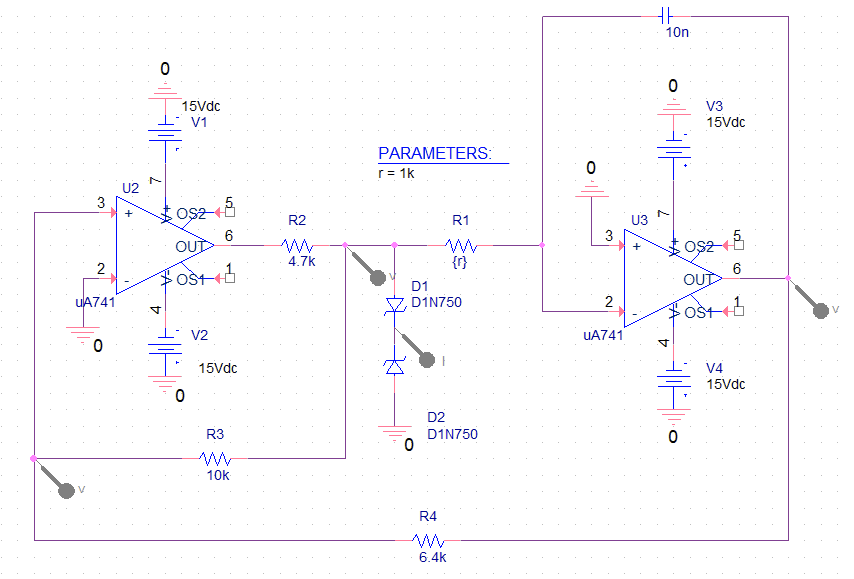
\includegraphics[width = \textwidth, height = .25\textheight, keepaspectratio]{lab/assets/exe1circuit.png}
	%\caption{Κύκλωμα προσομοίωσης τελεστικού ενισχυτή}
\end{figure}


\subsection{Ερώτημα 4}

\begin{figure}[h!]
	\centering
	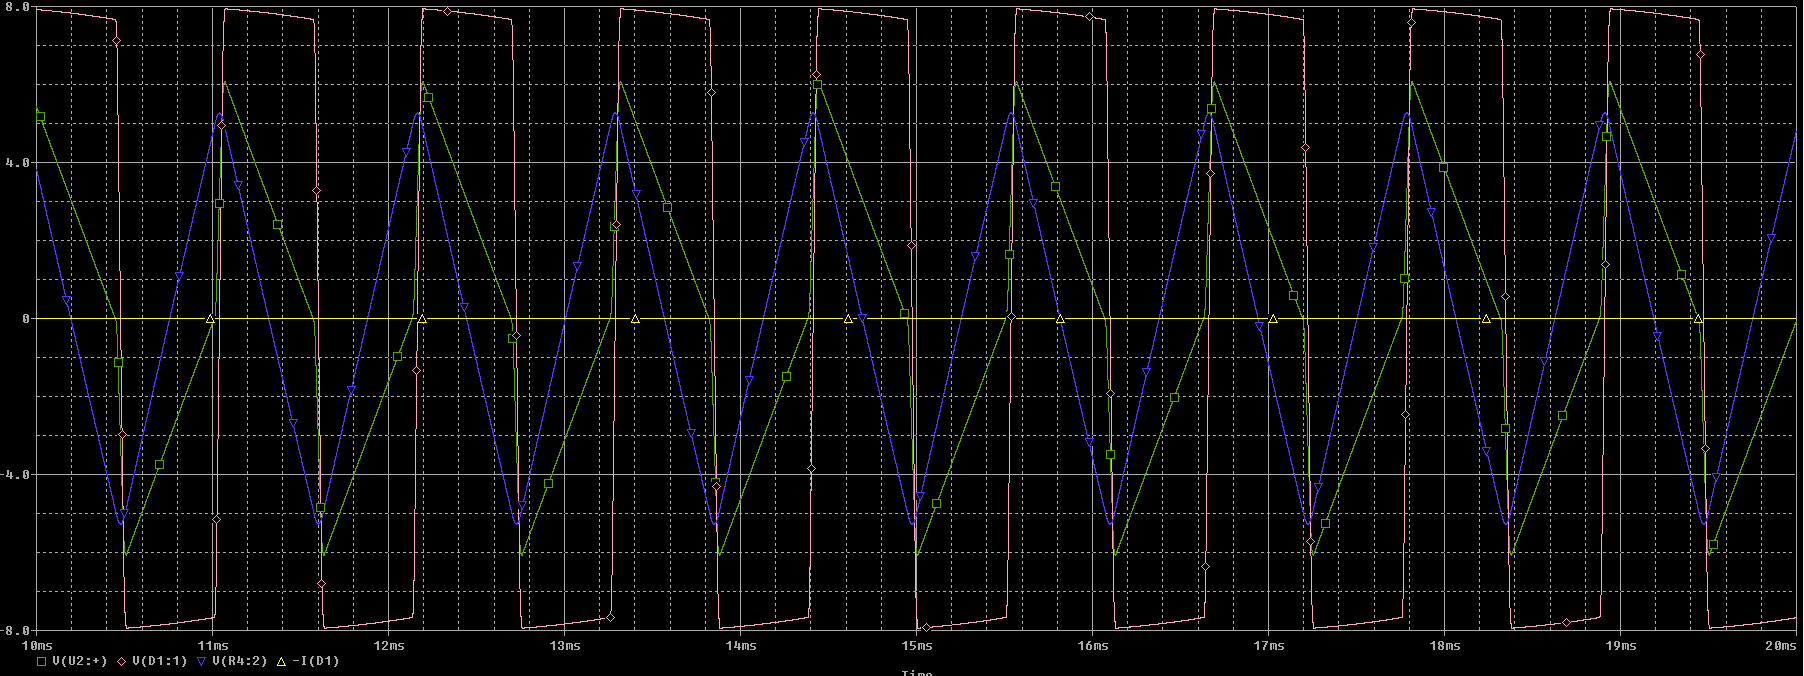
\includegraphics[width = \textwidth, height = .25\textheight, keepaspectratio]{lab/assets/gentri1.png}
	%\caption{Κύκλωμα προσομοίωσης τελεστικού ενισχυτή}
\end{figure}

\subsection{Ερώτημα 5}

\subsection{Ερώτημα 6}

\subsection{Ερώτηαμ 7}


\section{Άσκηση 2}


\end{document}